\documentclass[../report.tex]{subfiles}
\begin{document}
	
\subsection{PAA \& SAX}
	As described in the background section \cref{sec:paasax} on SAX, there are two steps.  PAA (Peicewise Aggregate Approximation) is applied before symbols are calculated based on equal breakpoints following a Gaussian distribution.
	
\subsubsection{Data Distribution} \label{sec:distribution}
	An assumption that is made by the SAX algorithm is that data is close to normally distributed  once it is \textit{Z-normalised} (\cref{sec:Z-normalisation}) to get an appropriate distribution of the symbols.  As can be seen from \cref{fig:dist_obs} which shows the distribution of data points over the whole observation in blue against a normal distribution in red, the whole data set is not a good fit for a normal distribution.

	However when data is only considered during an event as seen in \cref{fig:dist_evt} it can be seen that the data is a much closer fit.  Automated event detection is discussed in \cref{sec:eventdetection}.
	
\begin{figure}[H]
	\centering
	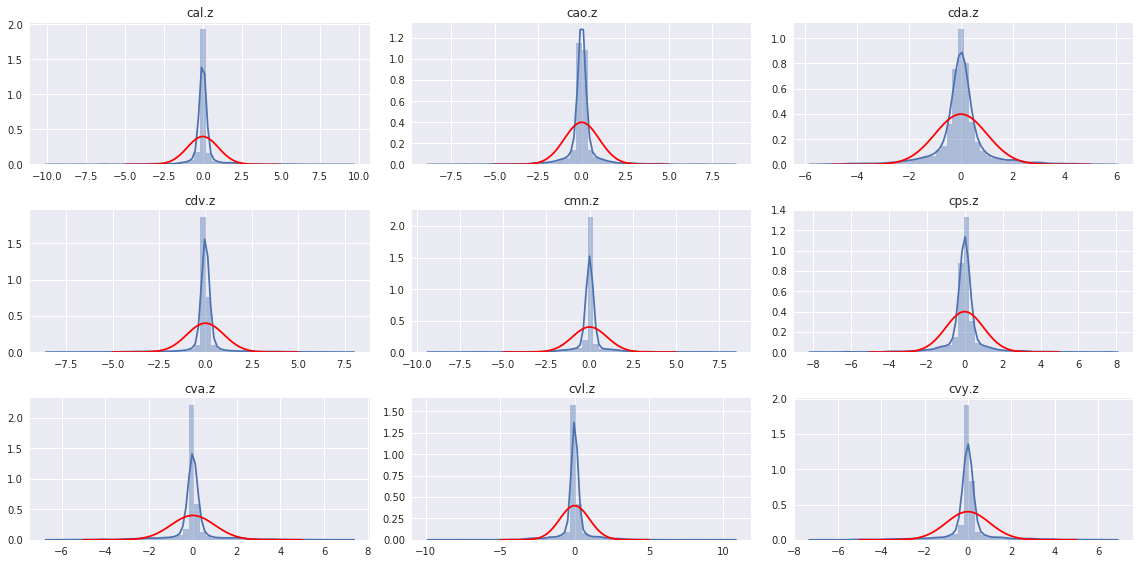
\includegraphics[width=1\linewidth]{img/distribution_obs}
	\caption{Distribution of Observation Data as a whole}
	\label{fig:dist_obs}
\end{figure}

\begin{figure}[H]
	\centering
	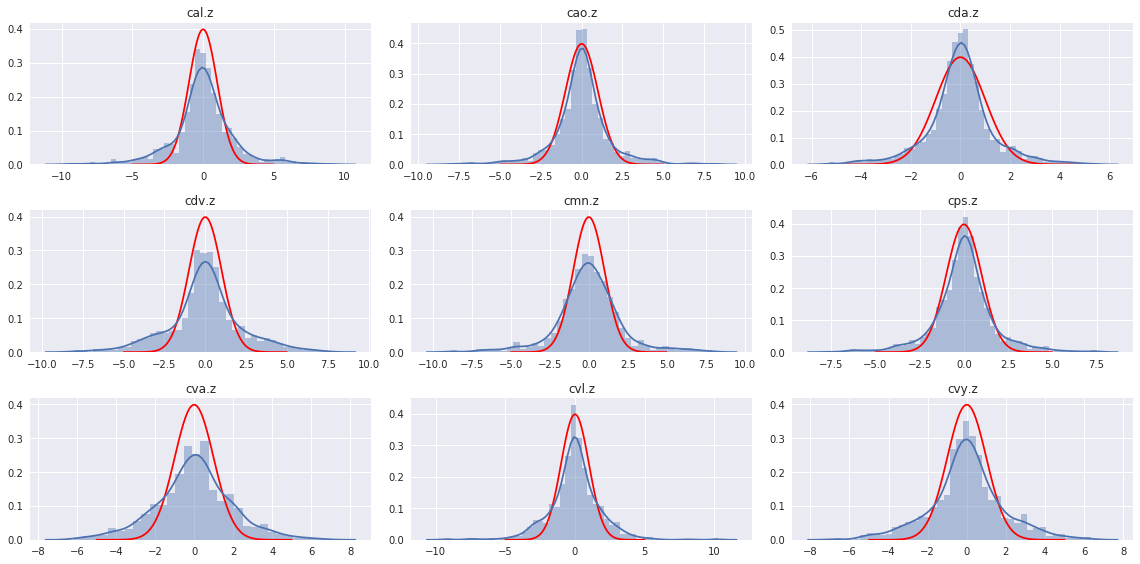
\includegraphics[width=1\linewidth]{img/distribution_evt}
	\caption{Distribution of Observation Data During an Event}
	\label{fig:dist_evt}
\end{figure}

	The disparity between the distributions can be attributed to the full observation traces including many data points during quiet periods that would naturally tend towards zero.  As the fit is significantly closer when only looking at data points during an event only, it suggests that a measure of the fit of a normal distribution may be a predictor to en event occurring.

\subsubsection{PAA}
	A Python class was written to be callable to convert a Dataframe into an array of the aggregated values.  To reduce the number of steps involved in using the class, it performs the normalisation step (unless told not to by passing \verb|normalise=False| as a parameter).
	
	\lstinputlisting[language=Python]{../seismic/sax/paa.py}
	
	When the class is first instantiated, a copy of the series is stored locally in the object.  Unless the normalise parameter is explicitly set to false, the numpy library is used to calculate the mean and standard deviation of the series and then $(x - \bar{x}) / \sigma$ is calculated for the whole series as described in \cref{sec:Z-normalisation}.
	
	This returns a callable object with the window size (in milliseconds) as a parameter.  When called, the object uses the resample feature of Pandas to return a series of mean values.	It should be defined and called as follows:
	
\begin{lstlisting}[language=Python]
	p = Paa(series=d)  # where d is a Pandas dataframe with a time index
	paa_out = p(50)    # performs PAA on d with a window size of 50ms
\end{lstlisting}

\subsubsection{SAX}
	Similar to the PAA class, the SAX class was written to produce a callable object.

	\lstinputlisting[language=Python]{../seismic/sax/sax.py}
	
	On instantiation, copy of the original series is stored in the object with no additional pre-processing.  The object is then called with the desired alphabet passed as the only parameter.  The length of the alphabet is used to determine the number of breakpoints to calculate against a normal distribution and these are stored as the \textit{thresholds}.  A Python generator is then returned that uses the numpy \textit{searchsorted} method to establish between which breakpoints a value falls and then return the corresponding character.  The generator can then be used to iterate over the values one at a time by the calling function.  A simple call to print the characters is demonstrated below:
	
\begin{lstlisting}[language=Python]
	s = Sax(paa_out)          # instantiate a callable Sax object
	for val in s("abcdefg"):  # iterate over the object
	    print(val, end="")    # print each value (with no newline)
\end{lstlisting}
	
\end{document}